%% https://tipp2021.triumf.ca/proceedings.html
%% Deadline 25 June 2021
%% 4 page maximum
\documentclass[a4paper]{jpconf}
\usepackage{graphicx}
\usepackage{lineno}
\usepackage[utf8]{inputenc} % Включаем поддержку UTF8
%\usepackage[russian,english]{babel}   % убрать русский перед отправкой статьи
\usepackage[pdftex, backref, colorlinks]{hyperref}
\usepackage{todonotes}
\usepackage{booktabs}
\pdfoutput=1 % if your are submitting a pdflatex (i.e. if you have
             % images in pdf, png or jpg format)

\graphicspath{{figures/}}
\bibliographystyle{iopart-num}

%%%%%%%%%%%%%%%%%%%%%%%%%%%%%%%%%%%%%%%%%%%%%%%%%
\begin{document}
%\linenumbers % Remove after editing
\newcommand{\todoi}[1]{\todo[inline]{\Russian #1}}
%\tableofcontents  % пусть пока побудет, стереть перед подачей
%\listoftodos[NotesToDo]

\title{Status of the SPHERE project for high energy cosmic ray studies by registering reflected Cherenkov light with a drone-borne detector}

\author[1]{D.~Chernov$^{1,\ast}$, 
E.~Bonvech$^{1}$, 
M.~Finger~Jr.$^{2,3}$, 
M.~Finger$^{2,3}$,
V.~Galkin$^{1,4}$, 
V.~Ivanov$^{4}$,
V.~Latypova$^{4}$,
D.~Podgrudkov$^{1,4}$, 
T.~Roganova$^{1}$ 
and I.~Vaiman$^{1}$.}

\address{$^1$ Lomonosov Moscow State University, Skobeltsyn Institute for Nuclear Physics, Moscow, Russian Federation}
\address{$^2$ Charles University, Faculty of Mathematics and Physics, 18000 Prague, Czech Republic}
\address{$^3$ Joint Institute for Nuclear Research, Dubna, Russian Federation}
\address{$^4$ Lomonosov Moscow State University, Faculty of Physics, Moscow, Russian Federation}
% e-mail addresses: only for the corresponding author
\ead{chr@dec1.sinp.msu.ru}

%\keywords{Cherenkov detectors, photon detectors for UV, visible and IR photons (Si-PMTs).}
%\arxivnumber{2005.07993} % only if you have one
%\proceeding{}

\begin{abstract}

Here we present the current state of the technical design of the SPHERE project’s new detector. The SPHERE project is aimed at primary cosmic ray studies in the 1--1000 PeV energy range using the reflected Cherenkov light method. The concept of a drone mounted detector with a photosensitive camera based on silicon photomultipliers is discussed. The design details of a small scale prototype of this detector is presented.    
\end{abstract}

\section{Introduction}
\label{sec:intro}

The SPHERE project is based on a technique proposed by Alexander Chudakov for primary cosmic ray studies~\cite{Chu74} by detection of  Cherenkov light (CL) reflected from the snow covered surface induced by extensive air showers (EAS). This approach was successfully implemented earlier in the SPHERE project\cite{Ant15a}, in particular in the experiments with the SPHERE-2 detector\cite{Ant20}. The small SPHERE--2 detector was carried by a tethered balloon above the snow covered Baikal lake (Russia). The experiment was carefully simulated~\cite{Ant19} and the resulting primary cosmic ray energy spectrum and the chemical composition data were published~\cite{Ant15c}. 

The main aim of the current stage of the SPHERE project (see Fig.~\ref{fig:DirectCL}) is to develop a new SPHERE-3 detector for primary cosmic ray mass composition studies in the energy range from 1 to 1000 PeV. The main features of the new detector are the silicon photomultipliers in the photosensitive camera and an unmanned aerial vehicle (UAV) as a detector carrier. 
\begin{figure}
    \begin{minipage}[b]{.45\textwidth}
    \centering 
        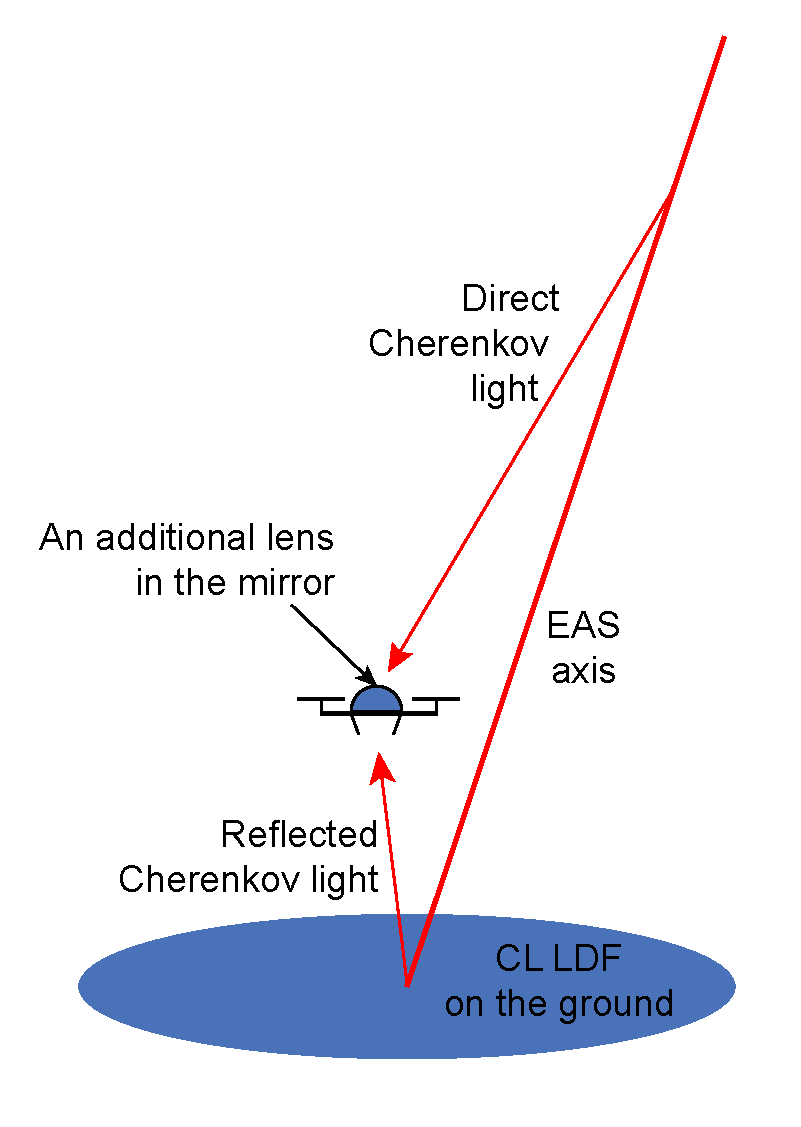
\includegraphics[height=.365\textheight]{DirectCL.pdf}
        \caption{Scheme of direct and reflected Cherenkov light from EAS.}
        \label{fig:DirectCL}
    \end{minipage}
    \hfill
    \begin{minipage}[b]{.52\textwidth}
        \includegraphics[height=.365\textheight, angle=-90]{Sphere3optic.eps}
        \includegraphics[height=.365\textheight, angle=-90]{Sphere3spot.eps}
        \caption{Preliminary version of the optical system with spot diagram analysis.}
        \label{fig:lightspots}
    \end{minipage}
\end{figure}

\begin{table}[b]
\centering
    \caption{Characteristics of the designed detectors.}
    \label{tab:statistics}
%\vspace{1pc}
    \begin{tabular}{ l c c}
        \toprule
        \textbf{Parameter}  & \parbox[t][.8cm]{3cm}{\centering{\textbf{Prototype of\\the detector}}} & \parbox[t][.8cm]{2cm}{\centering{\textbf{Target\\Detector}}} \\ [1.5ex]
        \midrule
        Effective aperture & 0,1 m$^2$ &  0.5 m$^2$\\ 
        Mirror diameter, up to & 80 cm &  160 cm\\
        Viewing angle of the optical system & $\pm$25$^\circ$ & $\pm$25$^\circ$ \\
        Number of pixels (SiPMs) & 133 &  up to 3000 \\
        Detector weight, up to &  10 kg &  50 kg \\
        Detector lifting height, up to &  500 m & 2000 m \\
        \bottomrule
    \end{tabular}
\end{table}

\begin{figure}[t]
\centering % \begin{center}/\end{center} takes some additional vertical space
\includegraphics[width=0.38\textwidth]{Fig2_1.pdf}
\hfill
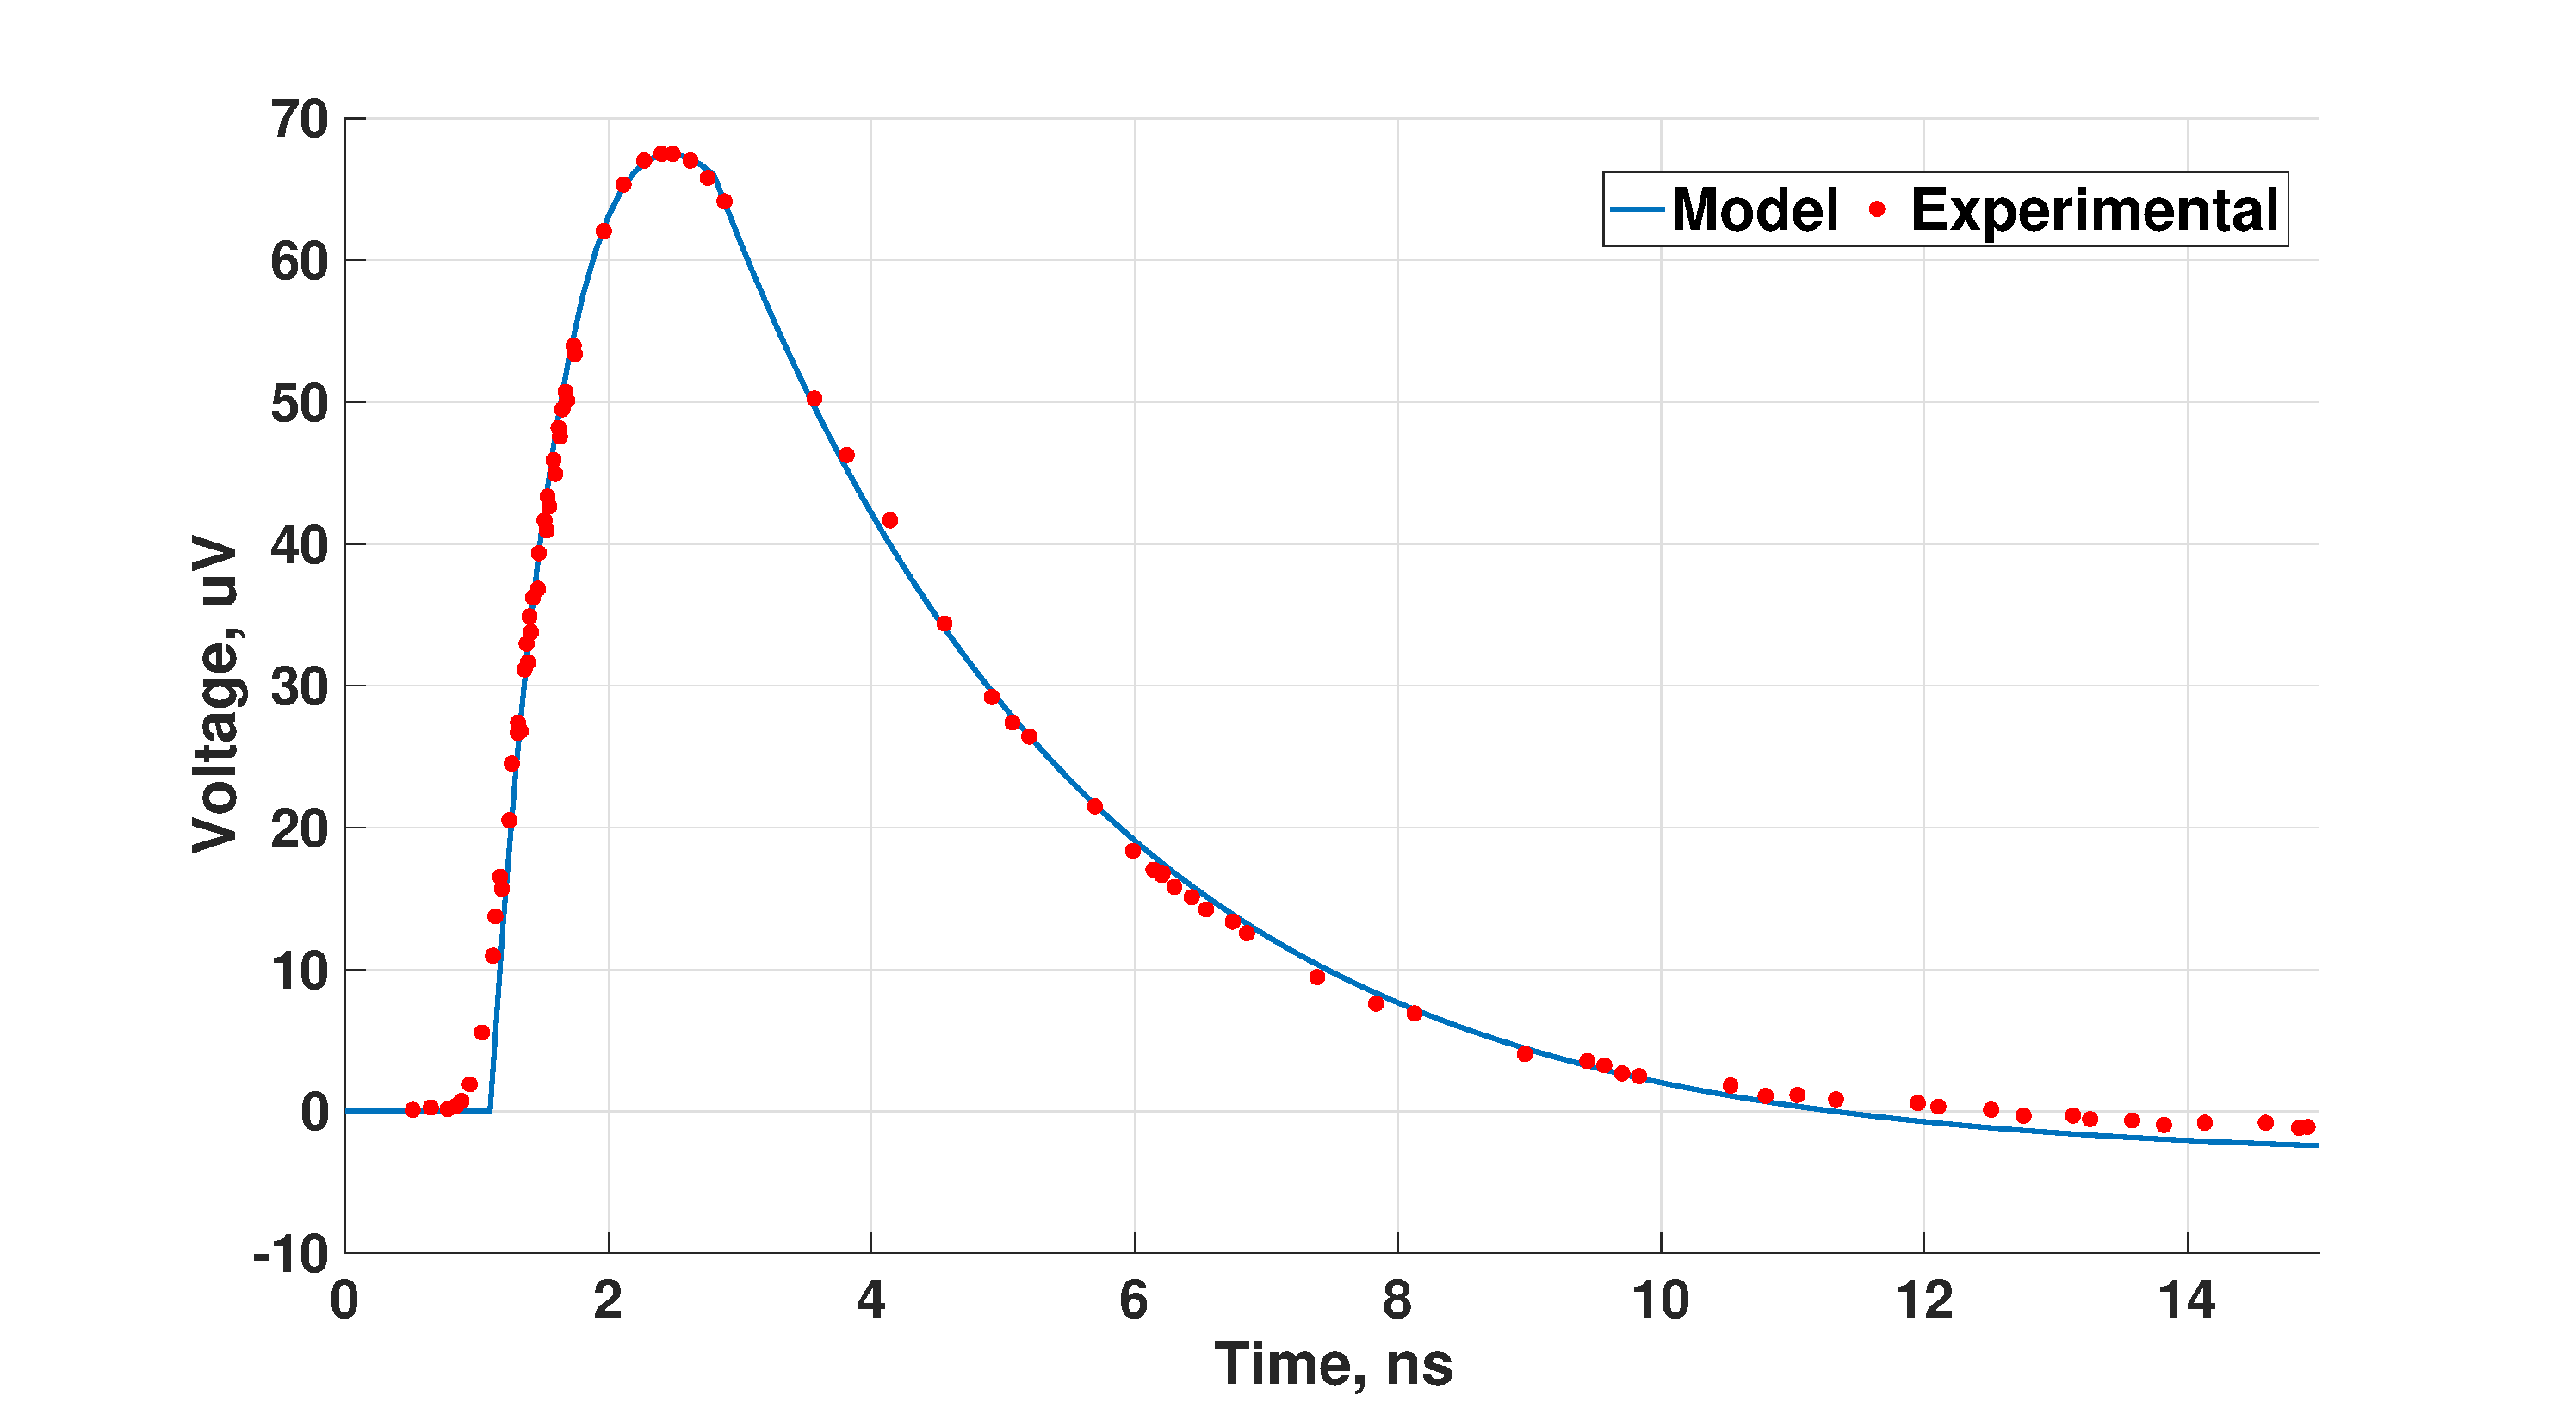
\includegraphics[width=0.60\textwidth]{The_pulse_shape_final.eps}
\caption{(Left) An electronic circuitry model approximating the real SiPM. The circuit model was built in MATLAB Simulink. (Right) The model curve of a current pulse from a single photoelectron obtained from MATLAB Simulink in comparison to the manufacturer provided data.}
\label{fig:Sphere_results}
\end{figure}


\section{Detector Design}
Preliminary design of the detector's prototype optical scheme is shown in Fig.~\ref{fig:lightspots}. The prototype viewing angle is $\pm$25$^\circ$. With 800~mm radius mirror and 460~mm aperture diameter the light spot on the sensitive surface is about 20~mm in diameter. Preliminary parameters of the detector and its prototype are given in Tab.~\ref{tab:statistics}.

The new detector will use the Schmidt optical system. The central part of the mirror will not be used since it is in the shadow of the photodetector. This area can be used to localise a system for the direct CL detection with an approximate aperture of 100 cm$^2$. Calculations show that for an EAS from a 1~PeV proton the CL photon density is $\sim$100 photons per cm at a distance of 100~m from the shower axis. Taking into account the SiPM quantum efficiency and losses on the optical elements the expected number of registered photoelectrons is around 1000.  Thus in addition to the data on the reflected CL information on the intensity and angular properties of direct CL can be used for estimating the mass of the primary particle. It is assumed that at the same primary energy and depth of EAS maximum an EAS from a primary proton should form a light spot different form that of a Fe nuclei.

\subsection{SiPM segment prototype }
The main sensitive element of the new detector will consist of 7-channel SiPM boards~\cite{TunkaSIT2020} based on the Micro FC-60035 SiPMs~\cite{SiPM_datasheet}. Tests of such boards were successfully completed. Each board was equipped with 7 pre-amplifiers and a temperature sensor. To increase the sensitivity of the detector we plan to adapt the SiPM boards to a wide angle optical scheme based on hemispherical lenses.

\subsection{SiPM modelling}
In order to increase the time resolution a fast output will be used for these SiPMs. But such output signals are distorted by negative afterpulses and overlapping of neighboring pulses. For higher estimation accuracy of photoelectron quantities we built a SiPM operation model. In Fig.~\ref{fig:Sphere_results} on the left the circuitry of the model SiPM is shown. The parameters were adjusted to emulate a manufacturer measured profile of a single photoelectron pulse. The model pulse profile (blue curve) along with the experimental data (red dots) is shown in Fig.~\ref{fig:Sphere_results} on the right.

\section{Experiment modeling}

The modeling procedure generally follows the approach used in the SPHERE-2 experiment. It includes event modeling and image processing.
Event modeling incorporates two stages: a) EAS simulation with the CORSIKA code including Cherenkov light generation and b) production of CL images of EAS events in the telescope mosaic. The 1st stage results in a detailed 3D-array of CL photoelecton distribution in spatial coordinates and arrival time on the snow for each EAS event. Photoelectons appear due to a special CORSIKA mode which allows to account the PMT efficiency during shower modeling. At the 2nd stage the shower cores are evenly spread on the snow over a 500 m radius circle centered under the telescope. Contributions from every patch of the CL spot on the snow to the signal on the mosaic PMTs are calculated on a photoelectron-by-photoelectron basis.

During processing the images are fitted with an axis-symmetric rational function. Then the approximations are integrated over the central circle and the surrounding ring. The ratio of these integrals is used as a criterion parameter for the separation of events by the primary mass. Criteria are optimized with respect to mass separation by varying the radii of the circle and the ring. Optimal criteria are obtained for different primary energies and zenith angles, detector elevation and atmosphere models (1 and 11 in CORSIKA terms).

\begin{figure}[t]
\centering 
    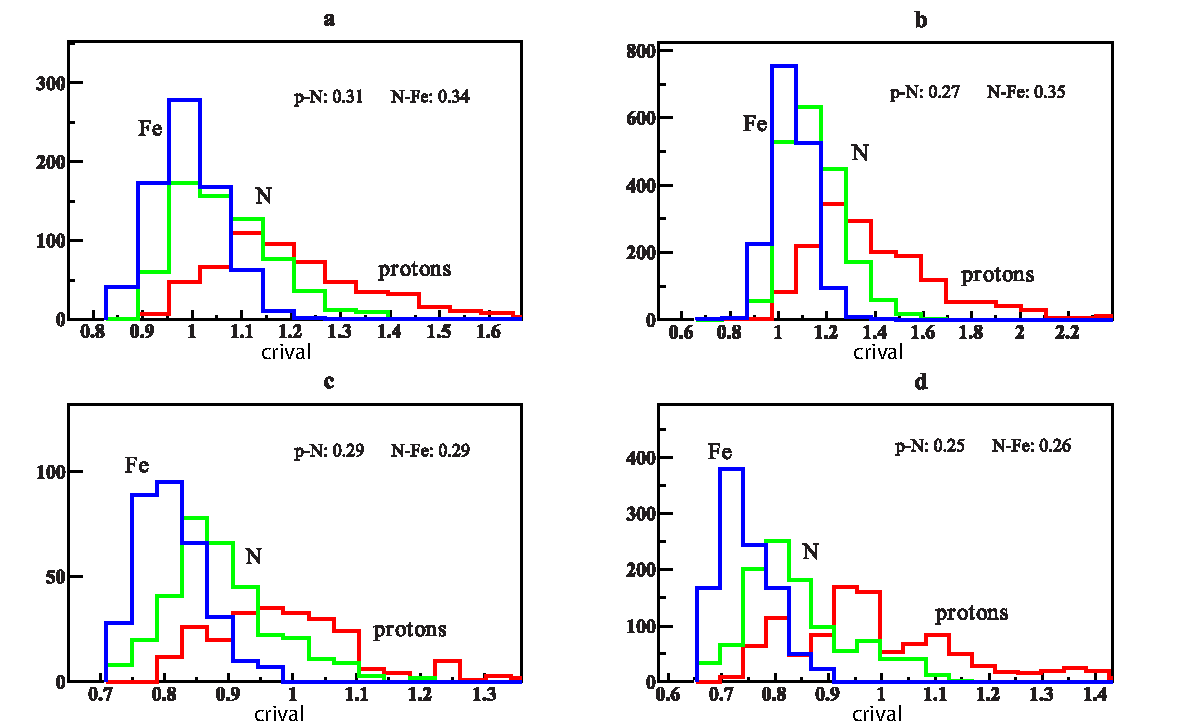
\includegraphics[width=0.75\textwidth]{poster.pdf}
    \caption{Criterion value distributions for p, N, Fe primaries. Zenith angle: $15^\circ$. Atmosphere model: 11. Figures inside the panels denote the probabilities of misclassification (classification errors) for pairs of primary particles p-N and N-Fe. \hspace{0.2cm}a,b --- $E_0$ = 10PeV, \hspace{0.2cm}c,d --- $E_0$ = 30PeV, \hspace{0.2cm}a,c --- h(elevation above the snow surface) = 500m, \hspace{0.2cm}b,d --- h = 900m.}
\label{fig:Modelling}
\end{figure}

Fig.~\ref{fig:Modelling} shows an example of primary mass criterion parameter distributions for p, N, Fe primaries made for the SPHERE-2 detector, since the optical design of the new detector has not yet been completed.

According to our previous work the use of direct CL angular distribution may help enhance the EAS separation by primary mass ~\cite{Gal18a}.

\section{Conclusion}
The development of a new SiPM based detector for EAS studies is continued. A prototype of a photosensitive matrix element has been developed and is being tested. The detector design and feasibility of some technical solutions are being studied.  For this purpose, a SiPM circuit model with a fast output was created. Analysis of the detector design performance for the mass composition studies is continued.

\section{Acknowledgments}
MEYS of Czech Republic grants LG14004 and LG18022.

\section*{References}
\bibliography{TIPP_Sphere}

\end{document}